\chapter[Resultados Obtidos]{Resultados Obtidos} \label{c3}

  Na primeira parte desse trabalho, foi implementado um protótipo com as condições mínimas para a execução do algoritmo de composição de contrapontos de primeira espécie. Para isso, foram implementados os módulos de notação musical, intervalos, escalas e contraponto. A execução dos testes é feita em uma função \textit{Main}.

  \section[Módulo de Notação Musical]{Módulo de Notação Musical}

    O módulo de notação musical possui quatro classes: \textit{Note}, \textit{Note Reader}, \textit{Compass Time} e \textit{Song}.

    \subsection[\textit{Note}]{\textit{Note}}

      A classe \textit{Note} é responsável pelo armazenamento das informações de uma nota. Os atributos de instância dessa classe são:

      \begin{enumerate}
        \item \textit{Duration}: número inteiro que representa a quantidade de tempo que a nota é tocada dentro de um compasso.
        \item \textit{Absolute Time}: número inteiro que indica a posição absoluta da nota na melodia, importante para contrapontos de segunda espécie em diante que utilizam da posição da nota no compasso.
        \item \textit{Note}: \textit{string} que armazena qual nota musical, entre A e G, ou R quando for uma pausa.
        \item \textit{Accidental}: \textit{string} que armazena os acidentes musicais que ocorrem à nota, se houver.
        \item \textit{Octave}: número inteiro que indica qual de qual oitava a nota é.
        \item \textit{MIDI Number}: número inteiro que representa a nota no formato padronizado MIDI, por exemplo, o Dó na quarta oitava é representado pelo número 72.
        \item \textit{Note Number}: número inteiro que representa a nota desconsiderando acidentes, utilizado para a classificação quantitativa de intervalos.
        \item \textit{Valid}: atributo booleano que indica se a nota é válida ou não, útil para retornar notas inválidas sem utilizar ponteiros, quando necessário.
      \end{enumerate}

      Além de construtores, a classe possui os seguintes métodos:

      \begin{enumerate}
        \item \textit{Full Note}: retorna uma \textit{string} representando a nota.
        \item \textit{Set Full Note}: constrói os outros atributos da uma nota a partir de uma \textit{string} padronizada, utilizada em construtores e outros métodos.
        \item \textit{Enarmonies}: retorna um vetor com as notas enarmônicas à nota do objeto.
      \end{enumerate}

      Por ser um protótipo, todos os atributos e métodos são públicos, isso será mudado na versão final, a Figura \ref{noteclass} descreve os atributos, métodos e construtores da classe.

      \begin{figure}[htb]
        \centering
        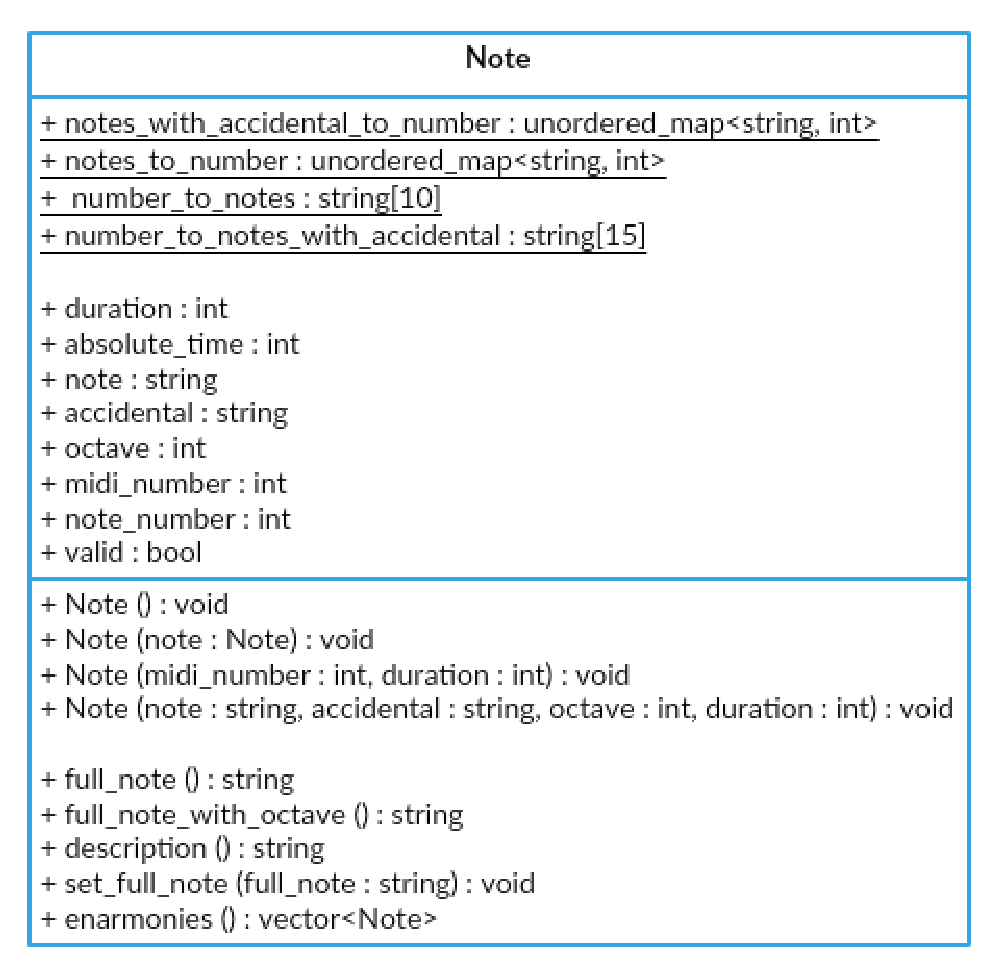
\includegraphics[scale=0.7]{figuras/noteclass.eps}
        \caption{Diagrama da Classe \textit{Note}}
        \label{noteclass}
      \end{figure}

    \subsection[\textit{Note Reader}]{\textit{Note Reader}}


      A classe \textit{Note Reader} é responsável pelo \textit{parser} de \textit{string} representado notas em formato Lilypond para instâncias da classe \textit{Note} e vice-versa. Sem a necessidade de atributos e com apenas métodos de classe, a classe age como uma biblioteca, sendo utilizada sem instanciação. Ela possui os seguintes métodos:


      \begin{enumerate}
        \item \textit{String To Note}: retorna uma instância de \textit{Note} ao receber uma \textit{string} e uma nota. A nota recebida como parâmetro é a nota anterior, pois o formato Lilypond omite a duração da nota se for a mesma da anterior.
        \item \textit{Note To String}: retorna uma \textit{string} que representa uma nota em formato Lilypond ao receber um objeto \textit{Note}.
        \item \textit{MSB}: retorna o bit mais significativo, utilizado no cálculo da figura musical baseado na duração da nota. Quanto maior for o valor da figura musical, menor a duração, mas pontos de aumento podem modificar a duração da nota e o bit mais significativo é usado para inferir o valor da figura musical, pois as figuras sem pontos de aumento sempre geram durações representadas por potências de 2.
        \item \textit{Number Of On Bits}: retorna o número de bits ligados de um inteiro, útil pois deriva o número de pontos de aumento de uma nota (para gerar a \textit{string}) a partir da representação binária da duração.
      \end{enumerate}

      A Figura \ref{notereaderclass} representa os métodos da classe.

      \begin{figure}[htb]
        \centering
        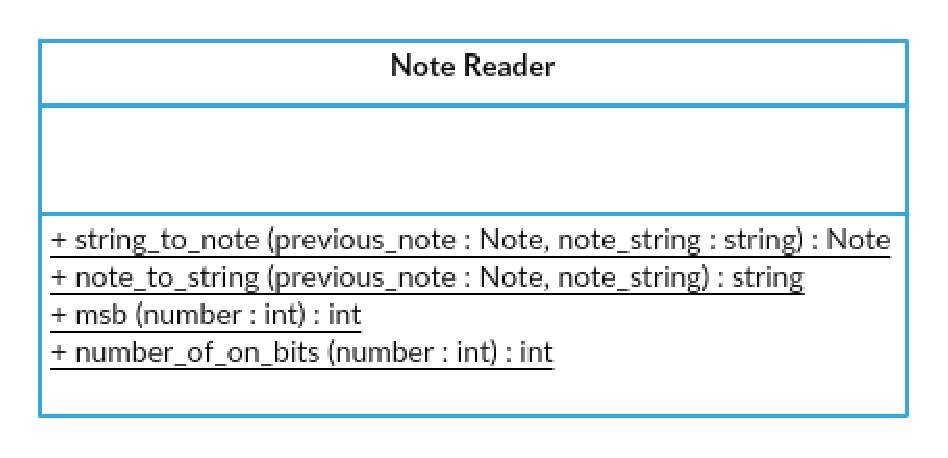
\includegraphics[scale=0.8]{figuras/notereaderclass.eps}
        \caption{Diagrama da Classe \textit{Note Reader}}
        \label{notereaderclass}
      \end{figure}

    \subsection[\textit{Compass Time}]{\textit{Compass Time}}

      A classe \textit{Compass Time} armazena o tempo de compasso de uma música. Possui os seguintes atributos:

      \begin{enumerate}
        \item \textit{Times}: Número inteiro, armazena a quantidade de batidas que o compasso possui, por exemplo, em um compasso 3/4, ele armazena o valor 3.
        \item \textit{Base Note}: Número inteiro, armazena qual é a figura musical base do compasso, por exemplo, em um compasso 3/4, ele armazena o valor 4.
      \end{enumerate}

      Além dos atributos, essa classe possui dois métodos:

      \begin{enumerate}
        \item \textit{Base Note Duration}: Retorna a duração da nota base.
        \item \textit{Compass Duration}: Retorna a duração total do compasso, multiplicando a duração da nota base pela quantidade de batidas.
      \end{enumerate}


      A Figura \ref{compasstimeclass} representa os atributos e métodos da classe.

      \begin{figure}[htb]
        \centering
        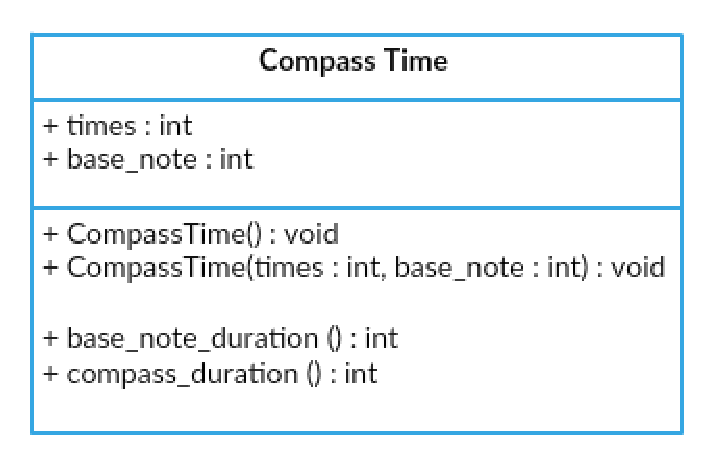
\includegraphics[scale=0.7]{figuras/compasstimeclass.eps}
        \caption{Diagrama da Classe \textit{Compass Time}}
        \label{compasstimeclass}
      \end{figure}

    \subsection[\textit{Song}]{\textit{Song}}

      A classe \textit{Song} armazena as informações básicas de uma música. Possui os seguintes atributos:

      \begin{enumerate}
        \item \textit{Notes}: Vetor que armazena as notas de uma música em ordem de execução.
        \item \textit{Scale}: Armazena a escala de uma música.
        \item \textit{Compass Time}: Armazena o tempo de compasso de uma música, assumindo que não há troca de tempo no meio da canção.
      \end{enumerate}

      Ela possui apenas um método chamado \textit{Size} que retorna o número de notas da música. A Figura \ref{songclass} representa os atributos e métodos da classe.

      \begin{figure}[htb]
        \centering
        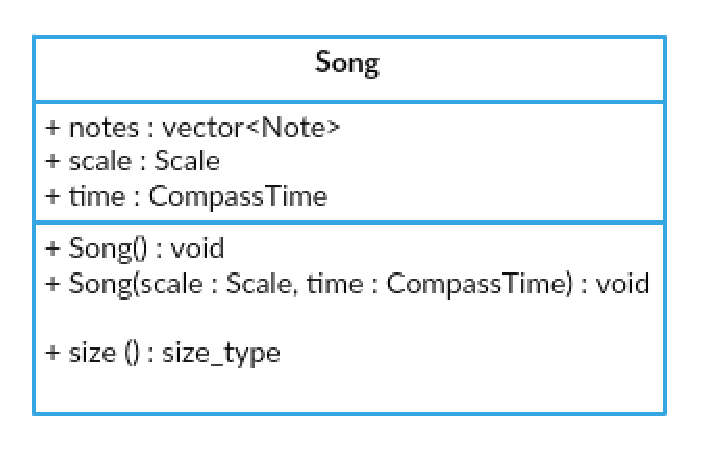
\includegraphics[scale=0.7]{figuras/songclass.eps}
        \caption{Diagrama da Classe \textit{Song}}
        \label{songclass}
      \end{figure}


  \section[Módulo de Intervalos]{Módulo de Intervalos}

    Responsável pela geração e armazenamento de intervalos, este módulo possui a classe \textit{Interval}.


    \subsection[\textit{Interval}]{\textit{Interval}}

      A classe \textit{Interval} armazena intervalos e possui método para gerar uma nota a partir de outra e um intervalos. Ela possui os seguintes atributos:

      \begin{enumerate}
        \item \textit{Quantitative}: número inteiro, representa a classificação quantitativa do intervalo.
        \item \textit{Qualitative}: \textit{string} que representa a classificação qualitativa do intervalo.
        \item \textit{Half Tones}: número inteiro, representa a quantidade de semitons característica do intervalo.
        \item \textit{Ascendant}: booleano que indica se o intervalo é ou não ascendente, no caso de intervalos melódicos.
      \end{enumerate}

      Excetuando-se métodos de impressão de atributos, a classe possui os seguintes métodos:

      \begin{enumerate}
        \item \textit{Is Dissonant}: retorna um booleano definindo se o intervalo é ou não dissonante, baseado nas regras do Contraponto Palestriniano.
        \item \textit{Is Consonant}: retorna um booleano definindo se o intervalo é ou não consonante.
        \item \textit{Interval to Note}: método de classe que retorna uma nota ao receber uma nota e um intervalo. A nota recebida é considerada a primeira ao utilizar a propriedade do intervalo ser ascendente ou descendente, pois uma nota e um intervalo sem atributo de ascendência pode gerar até duas notas, uma acima e outra abaixo da nota original.
      \end{enumerate}

      A Figura \ref{intervalclass} representa os atributos e métodos da classe.

      \begin{figure}[htb]
        \centering
        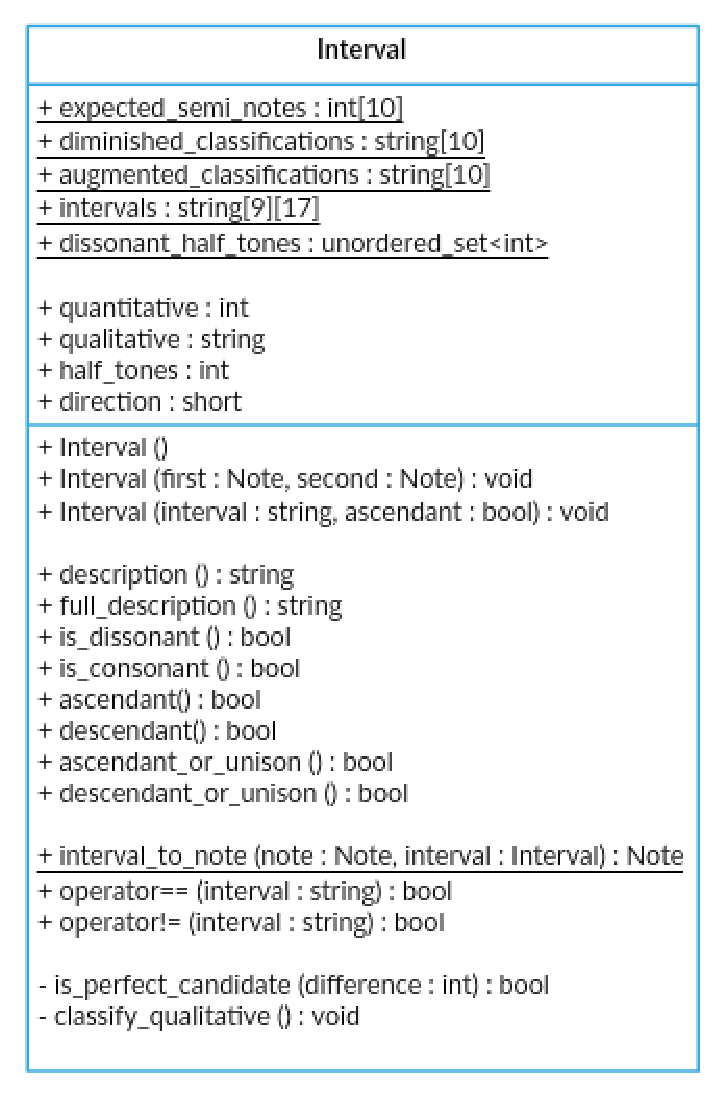
\includegraphics[scale=0.7]{figuras/intervalclass.eps}
        \caption{Diagrama da Classe \textit{Interval}}
        \label{intervalclass}
      \end{figure}

  \section[Módulo de Escalas]{Módulo de Escalas}

    O módulo de escalas é responsável pela geração e armazenamento de escalas musicais. Ele possui uma classe, a \textit{Scale}.

    \subsection[\textit{Scale}]{\textit{Scale}}

    A classe \textit{Scale} armazena as notas de uma escala, possuindo apenas um atributo, um \textit{set} de \textit{strings} chamado \textit{Permitted Notes} que define as notas permitidas para aquela escala. Além disso, ela possui os seguintes métodos:

    \begin{enumerate}
      \item \textit{Is Valid Note}: recebe uma nota e diz se ela está ou não presente na escala.
      \item \textit{Interval To Note On Scale}: método de classe que retorna uma nota, dado uma nota, um intervalo e uma escala. Retorna inválido se a nota não estiver presente na escala.
    \end{enumerate}


    A Figura \ref{scaleclass} representa os atributos e métodos da classe.

    \begin{figure}[htb]
      \centering
      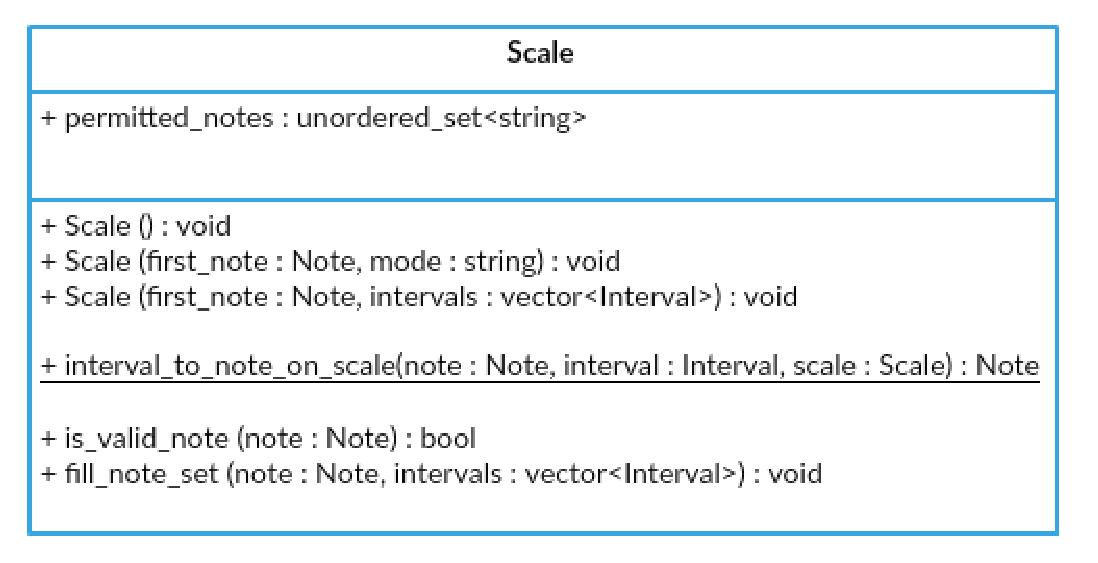
\includegraphics[scale=0.7]{figuras/scaleclass.eps}
      \caption{Diagrama da Classe \textit{Scale}}
      \label{scaleclass}
    \end{figure}

  \section[Módulo de Contraponto]{Módulo de Contraponto}

    O módulo de contraponto é responsável pela geração de contrapontos. Utilizando todas as classes anteriormente citadas, atualmente possui duas classes: \textit{Counterpoint} e  \textit{First Order Counterpoint}.

    \subsection[\textit{Counterpoint}]{\textit{Counterpoint}}

    A classe \textit{Counterpoint} funciona como uma biblioteca e não possui atributos de instância. Inicialmente utilizada para a implementação do contraponto de primeira ordem, atualmente possui o método ad-hoc de geração de contrapontos e o método de análise de notas para inserção no contraponto chamado \textit{Analyse and Add Interval}.

    A solução inicialmente concebida utiliza um algoritmo de seleção aleatório. Iniciando na primeira nota do \textit{cantus firmus}, monta-se um vetor de notas possíveis para o contraponto em seu estado atual, escolhe-se aleatoriamente uma das notas do vetor e a insere no vetor do contraponto, seguindo para a próxima nota. O vetor de notas possíveis era montado de acordo com as regras do contraponto de primeira espécie anteriormente citadas.

    O problema dessa solução era o fato de escolher randomicamente um caminho e não explorar os outros, o que podia levar a um caminho que não levava a uma solução. Para contornar isso, o algoritmo era rodado diversas vezes até se encontrar uma solução. Contudo, em músicas maiores o tempo de execução chegava a dois minutos ou mais, e em músicas impossíveis de se gerar contraponto, o algoritmo entrava em \textit{loop} infinito.

    Atualmente, essa classe é utilizada como classe pai da \textit{First Order Counterpoint} e será pai das classes dos contrapontos de outras espécies. A Figura \ref{counterpointclass} apresenta os métodos da classe.

    \begin{figure}[htb]
      \centering
      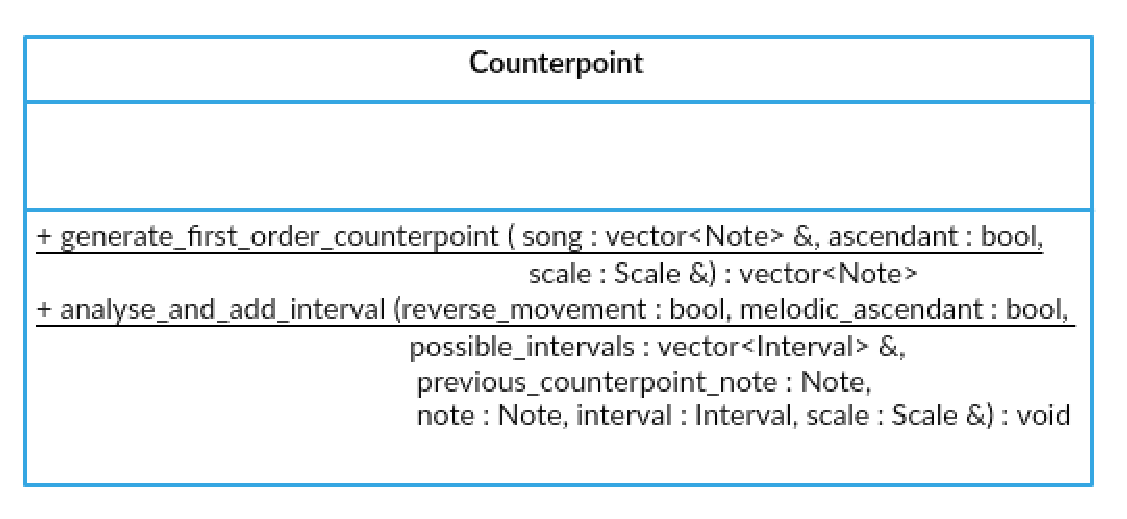
\includegraphics[scale=0.7]{figuras/counterpointclass.eps}
      \caption{Diagrama da Classe \textit{Counterpoint}}
      \label{counterpointclass}
    \end{figure}

    \subsection[\textit{First Order Counterpoint}]{\textit{First Order Counterpoint}}

      A classe \textit{First Order Counterpoint} herda da classe \textit{Counterpoint} e é uma biblioteca, possuindo atributos e métodos de classe. Possui os seguintes métodos:

      \begin{enumerate}
        \item \textit{DFS Generate Counterpoint}: recebe uma instância de \textit{Song}, um booleano que define se o contraponto será superior ou inferior e os números de terças e sextas paralelas e movimentos paralelos permitidos. Retorna um vetor de notas correspondente ao contraponto gerado.
        \item \textit{Solve}: Método recursivo que executa a busca completa para gerar contrapontos. Tem como parâmetros a posição atual no \textit{cantus firmus}, o número atual de terças ou sextas paralelas, o número de movimentos paralelos já ocorridos, a instância do \textit{cantus firmus} e da proposta de contraponto atual passadas por referência e um booleano indicando se o contraponto é inferior ou superior.
      \end{enumerate}

      O método que retorna o vetor de contrapontos encapsula a solução e chama o método recursivo. O algoritmo funciona da seguinta forma, iniciando na primeira posição do \textit{cantus firmus}, o estado da DP é definido por quatro parâmetros: posição, número MIDI da nota atual, número de terças ou sextas paralelas anteriormente executadas e número de movimentos paralelos.

      A transição ocorre após a geração do vetor de notas possíveis, de acordo com as regras do contraponto. Para cada nota do vetor de intervalos, adiciona-se a nota ao final do vetor de contrapontos se a inserção dela não fizer ultrapassar o número de terças, sextas e movimentos paralelos. Após a adição da nota, o método \textit{Solve} é chamado para a posição mais um, com o número de terças, sextas e movimentos paralelos atualizados. O retorno do método \textit{Solve} é um booleano que indica se há um contraponto válido ao explorar aquele caminho. Portanto, se o retorno for \textit{false}, a nota adicionada no final do vetor de contrapontos é removida e a próxima nota do vetor de notas possíveis é testada. Contudo, se o retorno for \textit{true}, ela também retorna \textit{true} e não remove a nota atual, mantendo o vetor de contraponto gerado como solução. Se a análise das notas não adicionar nenhuma nota no vetor de notas possíveis, o método retorna também \textit{false}. Vale ressaltar que o vetor de notas possíveis é embaralhado aleatoriamente para garantir uma solução diferente a cada execução do algoritmo. Além disso, primeiro adiciona-se as notas que geram movimento contrário, embaralha-se a primeira parte do vetor, em seguida, adiciona-se as notas que geram movimento paralelo e embaralha-se a segunda parte do vetor. Isso é feito para que a solução priorize o menor número de movimentos paralelos possível.

      O caso-base da DP é quando a posição é maior que o tamanho do \textit{cantus firmus}. Se o algoritmo chegar a essa posição, significa que a proposta de contraponto atual é um contraponto válido, portanto, retorna-se \textit{true}.

      Para que o algoritmo funcione efetivamente como uma DP, é utilizado um vetor de memorização, sendo um atributo de classe, é um vetor booleano de quatro dimensões, uma para cada estado. A primeira possui 201 espaços, permitindo que um contraponto seja gerado para um \textit{cantus firmus} com, no máximo, 201 notas. A segunda dimensão possui 90 espaços e representa o número MIDI da nota atual e cobre as 88 primeiras notas do piano. A terceira dimensão possui 5 espaços e cobre as 4 terças ou sextas paralelas seguidas permitidas pelo algoritmo. A quarta dimensão representa o número de movimentos paralelos que aconteceram durante o contraponto, possui 100 espaços pois o máximo de movimentos paralelos permitidos pelo algoritmo é metade do tamanho do contraponto ou menos.

      Utilizando o vetor de DP, ele inicia todas as posições com \textit{true}. Quando o algoritmo encontra um estado que é não possui solução, memoriza como \textit{false} na posição do vetor de DP que representa aquele e todas as posteriores consultas àquele estado retornam falso sem explorar esse candidato de solução novamente. Um exemplo é se o algoritmo definir que o estado atual -- na posição 10, na nota C4 (\textit{MIDI number} 60), com 2 terças ou sextas paralelas e 13 movimentos paralelos -- não é uma solução, memoriza-se \textit{false} em dp[10][60][2][13]. Na próxima consulta a esse estado, retorna falso imediatamente sem explorar. Memorizar estados que retornam \textit{true} é irrelevante pois o primeiro estado completo que chega ao final retornando \textit{true} é definido como a solução.

      A Figura \ref{firstordercounterpointclass} apresenta os métodos e atributos da classe.

      \begin{figure}[htb]
        \centering
        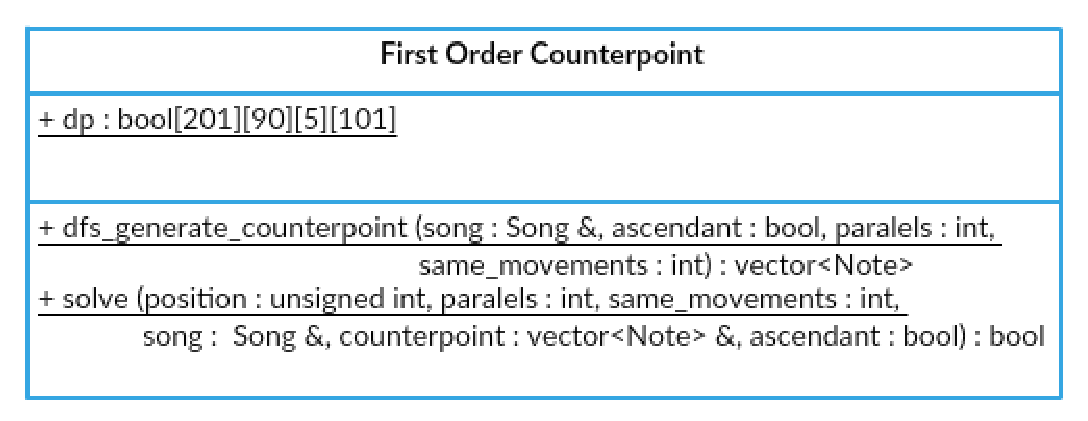
\includegraphics[scale=0.7]{figuras/firstordercounterpointclass.eps}
        \caption{Diagrama da Classe \textit{First Order Counterpoint}}
        \label{firstordercounterpointclass}
      \end{figure}


  \section[\textit{Main}]{\textit{Main}}

    A \textit{Main} é a função principal que executa o programa. Nela o arquivo .ly é lido -- primeiramente lendo a tônica e o modo da escala, seguido pela leitura do ritmo. Após isso, cada nota é lida e convertida para uma instância de \textit{Note} por meio da \textit{Note Reader}. Para efeitos de teste, atualmente, os intervalos melódicos são calculados e impressos no terminal, bem como a transformação de \textit{Note} para \textit{string} novamente.

    Após a leitura, o algoritmo de contraponto é executado. É gerado um vetor de notas com o contraponto de primeira espécie. Esse vetor é impresso no terminal em notação musical padrão e em notação específica do Lilypond para fácil transferência do contraponto para o arquivo original.

  \section[Experimentos]{Experimentos}

    Para validar os algoritmo construído, foram feitos experimentos em músicas pequenas para melhor análise do resultado. O teste da execução do algoritmo foi feito utilizando várias músicas. Serão apresentados os testes feitos com a música infantil \textit{Twinkle Twinkle Little Star}. O código-fonte da solução está disponível em \textit{\url{https://github.com/joao18araujo/ly_parser}}.

    A música original pode ser observada em formato Lilypond e em pártitura no código \ref{twinklecode} e na figura \ref{twinkleoriginal}, respectivamente.

    \begin{lstlisting}[language={C}, caption={\textit{Twinkle Twinkle Little Star}}, label={twinklecode}]
    \key c \major
    \time 4/4
    c''4 c'' g'' g''
    a'' a'' g''2
    f''4 f'' e'' e''
    d'' d'' c''2
    g''4 g'' f'' f''
    e'' e'' d''2
    g''4 g'' f'' f''
    e'' e'' d''2
    c''4 c'' g'' g''
    a'' a'' g''2
    f''4 f'' e'' e''
    d'' d'' c''2
    \end{lstlisting}

    \begin{figure}[htb]
      \centering
      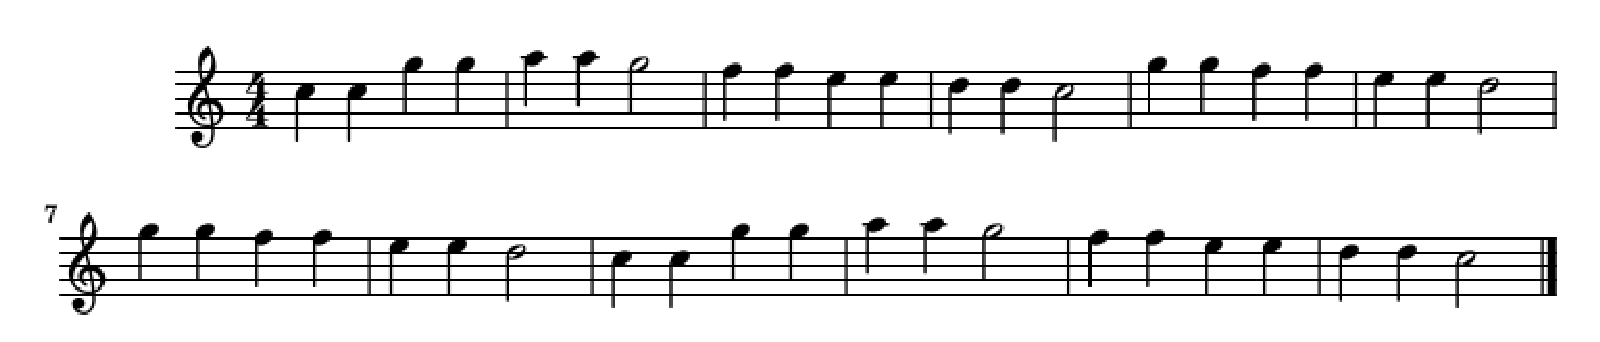
\includegraphics[scale=0.6]{figuras/twinkleoriginal.eps}
      \caption{Partitura de \textit{Twinkle Twinkle Little Star}}
      \label{twinkleoriginal}
    \end{figure}

    Após a primeira execução do algoritmo, o contraponto gerado pode ser visto em formato Lilypond no código \ref{cont1.1} e em partitura na Figura \ref{cont1.2}.

    \begin{lstlisting}[caption={Primeiro contraponto gerado}, label={cont1.1}]
      c''4 c'4 e'4 e''4
      c''4 f''4 e''2 d''4
      d''4 c''4 g'4 b'4
      f'4 a'2 g'4 b'4
      d''4 d'4 c''4 g'4
      b'2 g'4 b'4 d''4
      d'4 c''4 g'4 d'2
      a'4 e'4 e'4 b'4
      a'4 c''4 g'2 d''4
      d'4 e'4 g'4 b'4
      f'4 c''2
    \end{lstlisting}

    \begin{figure}[htb]
      \centering
      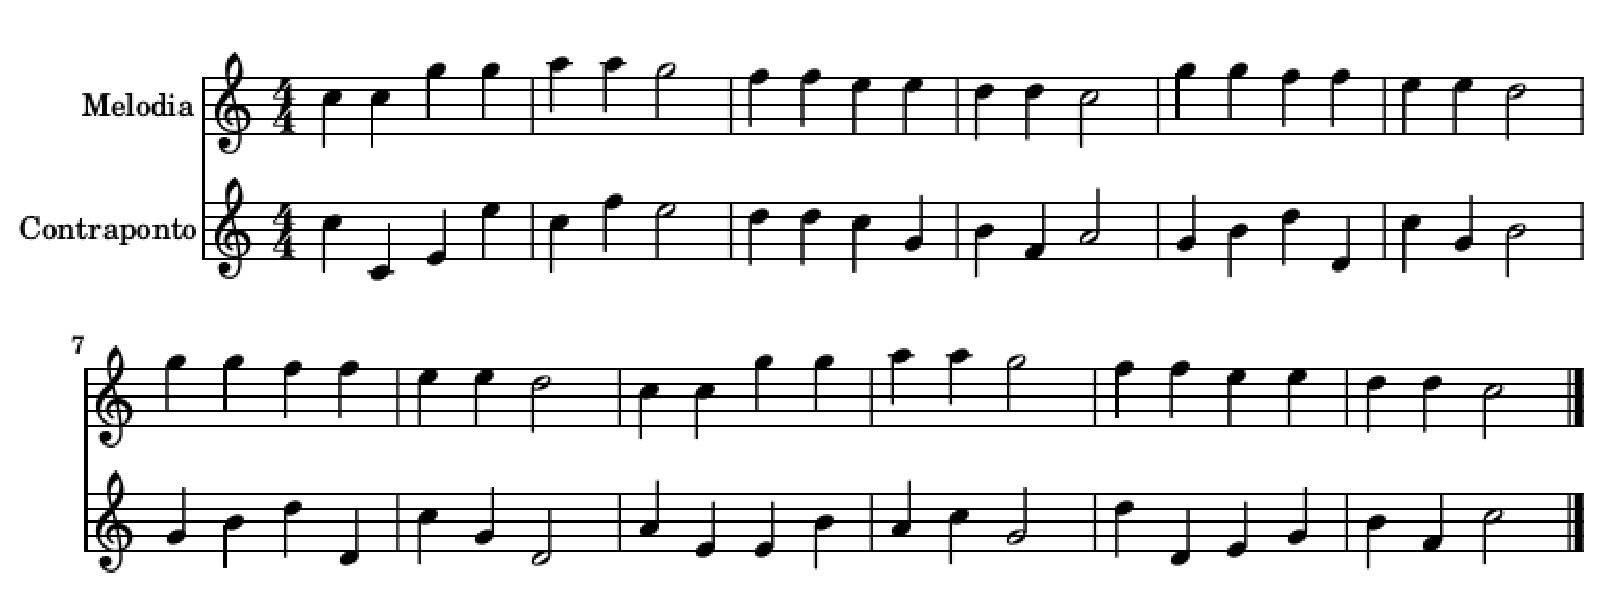
\includegraphics[scale=0.6]{figuras/cont1.2.eps}
      \caption{Partitura do primeiro contraponto gerado}
      \label{cont1.2}
    \end{figure}

    Após a segunda execução do algoritmo, o contraponto gerado pode ser visto em formato Lilypond no código \ref{cont2.1} e em partitura na Figura \ref{cont2.2}.

    \begin{lstlisting}[caption={Segundo contraponto gerado}, label={cont2.1}]
      c'4 e'4 e'4 e''4
      f'4 f''4 e''2 d''4
      d''4 c''4 g'4 b'4
      f'4 a'2 e'4 g'4
      d''4 d'4 g'4 e'4
      f'2 e'4 g'4 d''4
      d'4 g'4 e'4 f'2
      a'4 e'4 e'4 e''4
      a'4 c''4 g'2 a'4
      f'4 g'4 e'4 b'4
      f'4 c''2
    \end{lstlisting}

    \begin{figure}[htb]
      \centering
      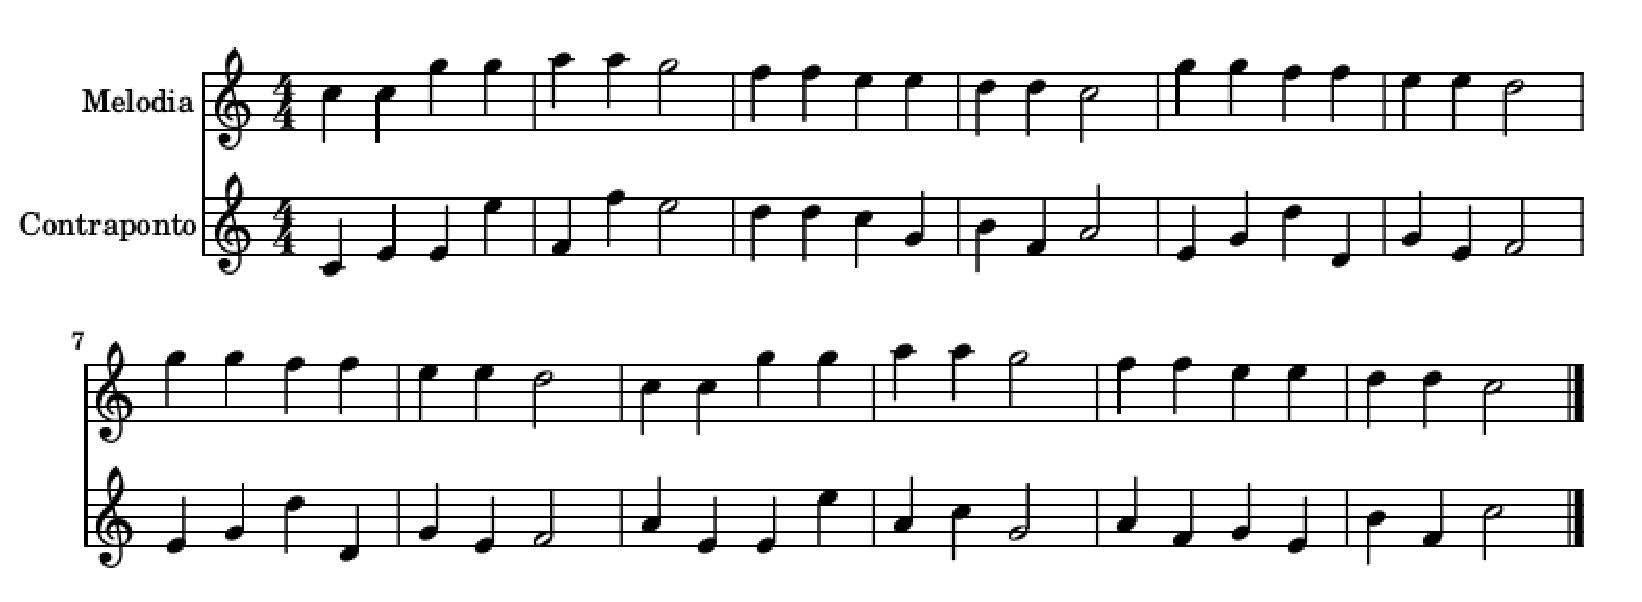
\includegraphics[scale=0.6]{figuras/cont2.2.eps}
      \caption{Partitura do segundo contraponto gerado}
      \label{cont2.2}
    \end{figure}

    Após a terceira execução do algoritmo, o contraponto gerado pode ser visto em formato Lilypond no código \ref{cont3.1} e em partitura na Figura \ref{cont3.2}.

    \begin{lstlisting}[caption={Terceiro contraponto gerado}, label={cont3.1}]
      c''4 a'4 e'4 e''4
      f'4 a'4 b'2 d''4
      d''4 c''4 g'4 b'4
      f'4 a'2 g'4 b'4
      d''4 a'4 c''4 g'4
      b'2 g'4 b'4 d''4
      d'4 c''4 c'4 d'2
      e'4 a'4 e'4 b'4
      a'4 c''4 e''2 d''4
      d'4 c''4 c'4 b'4
      b'4 c''2
    \end{lstlisting}

    \begin{figure}[htb]
      \centering
      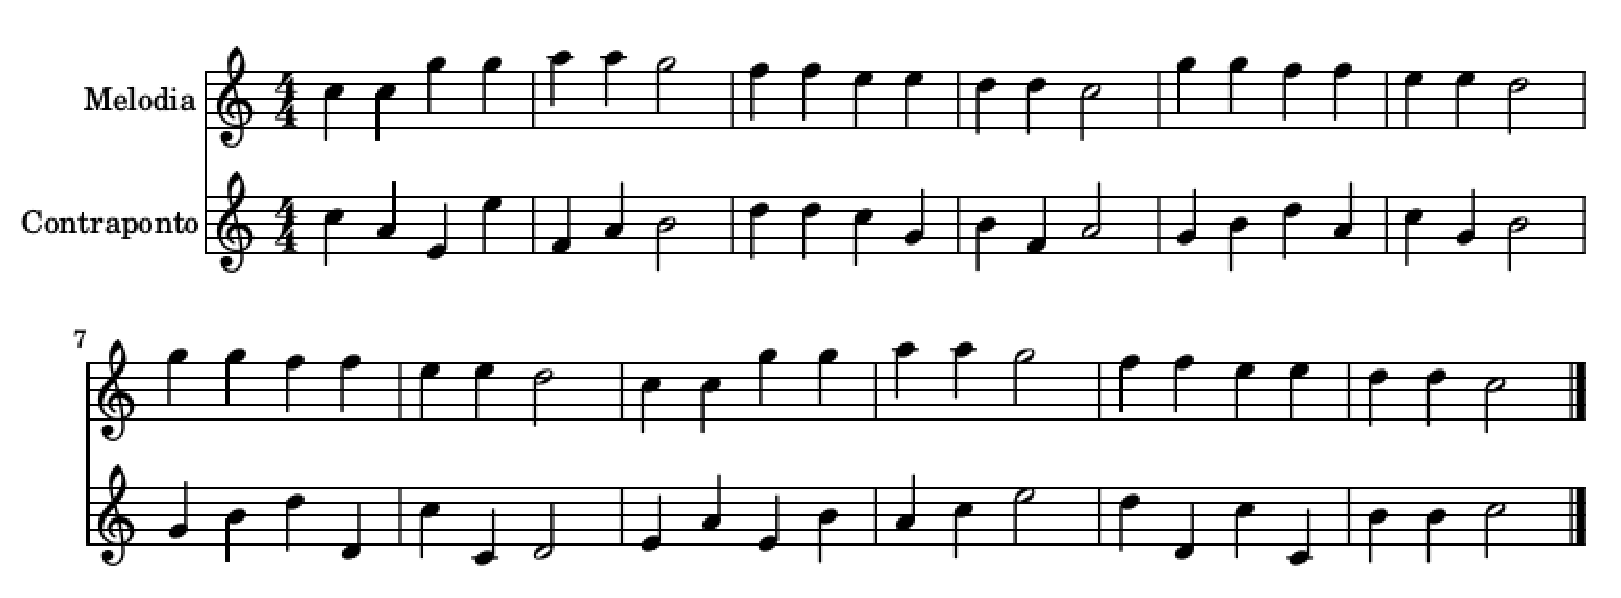
\includegraphics[scale=0.6]{figuras/cont3.2.eps}
      \caption{Partitura do terceiro contraponto gerado}
      \label{cont3.2}
    \end{figure}
